\lecture{2}{10/10}

A note on notation, we may use $S^\star$ to denote a finite length tuple containing only elements in $S$. This is not the same as the complex analysis definition where $\C^\star = \C \setminus \{0\}$. For example, $(0, 0, 1, 1, 0 ,1) \in \{ 0, 1 \}^\star$.

\begin{definition}[]
    A language $\mathcal L$ is \textbf{Turing-Recognisable} if there exists a turing machine $\mathcal M$ that recognises it. That is, $\mathcal L = L(\mathcal M)$.
\end{definition}

\begin{definition}[]
    A language $\mathcal L$ is \textbf{Turing-Decideable} if there exists a turing machine $\mathcal M$ that accepts all $w \in \mathcal L$ and rejects all $w \not \in \mathcal L$.
\end{definition}

So we say that $\mathcal M$ recognises $\mathcal L$ if it accepts every word in $\mathcal L$, but $\mathcal M$ decides $\mathcal L$ if it accepts every word and rejects every word not in $\mathcal L$.

You may see the terminology `r.e.' (stands for \textbf{recursively enumerable}) instead of Turing-Recognisable and \textbf{recursive} instead of Turing-Decidable.

\begin{remark}
    The set of all turing machines is countable, we will return to this.
\end{remark}

\begin{definition}[Multitape turing machines]
    A \textbf{multitape turing machine} is the same as a regular turing machine with several tapes, each of them having its own head. In the formal definition, we have the following transition function \[ \delta : Q \times \Gamma^k \to Q \times \Gamma^k \times \{ L, R \}^k. \] 
\end{definition}

\begin{theorem}[]
    Every multiple tape turing machine has an equivalent single tape turing machine.
\end{theorem}

\begin{proof}
    Say we have $k$ tapes $w_1, w_2, \ldots, w_k$. We then consider the tape \[w_1 + \# + w_2 + \# + \ldots + \# + w_k.\] So we have each tape delimited by a special character $\#$. We then alter our alphabet slightly. Consider $\Gamma$ as the alphabet of the single tapes. Then the alphabet for our multitape is $\Gamma'$ where $\Gamma \subset \Gamma'$ and \[ \; \forall \; \gamma \in \Gamma \; \exists \; \gamma' \in \Gamma'\] where $\gamma'$ is a special copy of each symbol used to represent the head in the multitape for each individual tape. We must now modify our transistion function to handle the movement between tapes. But here, we are at the point where a single tape turing machine now replicates a multitape turing machine.
\end{proof}

This proof shows how we talk about Turing machines. We do not need to be rigorous (although we can) in these proofs, and we build upon previous theorems a lot in our proofs. So we know now that if we can find a multitape Turing machine that can execute something, we can find a single tape Turing machine to do the same thing.

\begin{definition}[]
    A \textbf{non-deterministic turing machine} has a transition function of the form \[ \delta: Q \times \Gamma \to \mathcal P(Q \times \Gamma \times \{L, R\}) \] where $\mathcal P$ represents the power set function.
\end{definition}

\begin{figure}
    \centering
    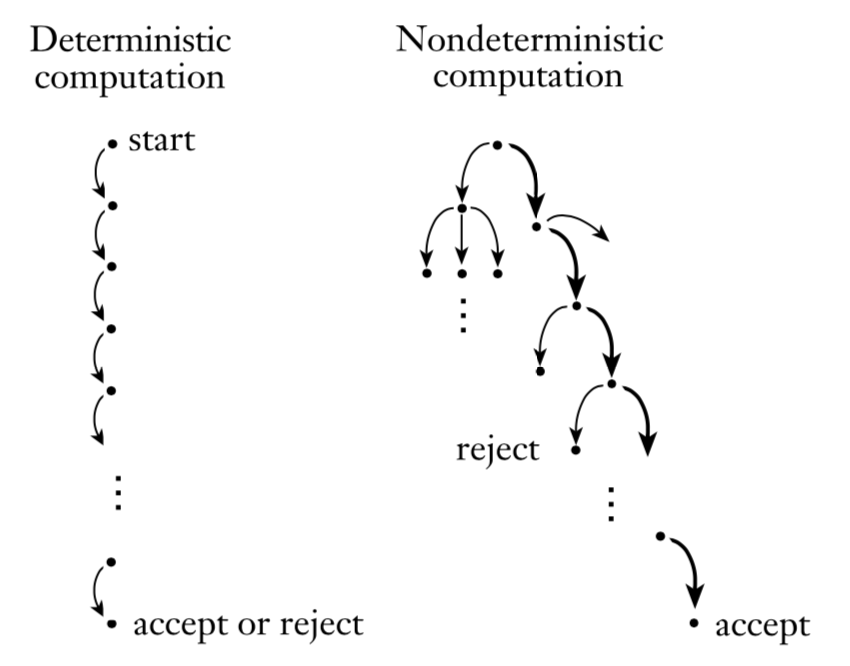
\includegraphics[width = 0.5\textwidth]{images/non-deterministic-turing-machine.png}
    \caption{Deterministic and non-deterministic Turing machine tree diagram.}
    \label{fig:non-deterministic-turing-machine}
\end{figure}

You can see a graphical representation of a non-deterministic Turing machine compared to a deterministic one. Informally, in a non-deterministic Turing machine there may exist several choices for the next state (and movement / writing of the head).

\begin{theorem}[]
    Every non-deterministic turing machine has an equivalent deterministic turing machine.
\end{theorem}

\begin{proof}
    The general idea for this proof is to consider the tree of all possible computations of a non-deterministic turing machine. We start from the root and do a breadth-first search and accept only if an accepting configuration is found. This can be done on a multitape turing machine, and hence there exists an equivalent deterministic turing machine.
\end{proof}
